\documentclass{article}

\usepackage{graphicx}
\usepackage{float}
\usepackage{makecell}
\usepackage[bottom]{footmisc}

% Enter the name of the subject
\newcommand{\assignmentname}{Project report}
% Your names
\newcommand{\studentA}{ACED}

\title{\textmd{\textbf{Dissertation}}\\\normalsize\vspace{0.1in}\Large{\assignmentname}\\\vspace{0.1in}\small{\textit{3 Ba INF \  2018-2019}}}
\author{\studentA}
\date{}

\begin{document}
\maketitle

\section{Introduction}
In this report we will look at the effects of expanding the simulated area. Previously, the simulations were limited to Flanders, this paper will compare the previous results to those aqcuired using simulations for (a large part) of Belgium. We will first look at the individual simulation results for Flanders and Belgium using a predetermined configuration. Then we will attempt to draw meaningful conclusions from the observed differences or similarities between them. \\
For both Belgium and Flanders we have simulated a 'standard' scenario 1000 times in order to acquire a representative baseline for comparison. This scenario uses the measles disease profile with $R_0$ = 11, immunity rate = 80\% and a population of 600,000 over 300 days. This is based on the scenario used in the stochastic variation tests in the simulation paper. Participation partitions are as follows
\begin{itemize}
	\item College = 0.5
	\item Workplace = 0.75
	\item Daycare = 0.45
	\item Preschool = 0.99
\end{itemize} 
The sections below will detail the results.

\section{Belgium}
\subsection{Plots}

\begin{figure}
	\centering
	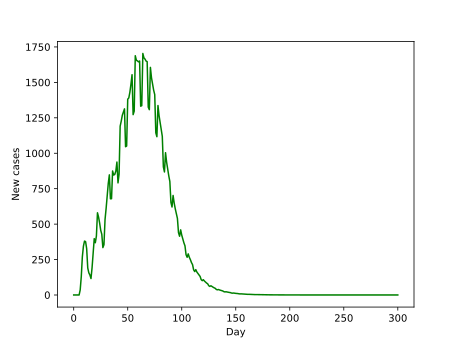
\includegraphics[width=\linewidth]{./Belgie/AVG_SR=0.002.svg}
	\label{Belgie-AVG_SR02}
	\caption{Average new cases per day. Seeding rate = 0.2\%, $R_0$ = 11, immunity rate = 80\%}
\end{figure}

\subsection{Stats}

\subsection{Conclusions}


\section{Flanders}
\subsection{Plots}

\subsection{Stats}

\subsection{Conclusions}

\section{Comparison}
\subsection{Plots}

\subsection{Stats}

\subsection{Conclusions}

\end{document}